\documentclass[numbers=noendperiod]{scrartcl}
\usepackage[utf8]{luainputenc}
\usepackage[T1]{fontenc}
\usepackage[ngerman]{babel}
\usepackage[a4paper,margin=0.75in, bottom=1in]{geometry}
\usepackage{enumerate}
\usepackage{minted}
\usepackage{mdframed}
\usepackage{courier}
\usepackage{hyperref}
\usepackage{graphicx}
\usepackage{subcaption}

\begin{document}
	
	\definecolor{bg}{RGB}{230,230,230}
	\newcommand{\inputmintedframed}[2]{
		\begin{mdframed}[linecolor=bg,backgroundcolor=bg]
			\inputminted[mathescape,breaklines,linenos,numbersep=5pt,tabsize=3]{#1}{#2}
	\end{mdframed}}
	
	\hrulefill
	\begin{center}
		\bfseries % Fettdruck einschalten
		\sffamily % Serifenlose Schrift
		\begin{huge}
			Betriebs- und Kommunikationssysteme
		\end{huge}\\
		\begin{Large}
			Sommersemester 2017, 5. Übungsblatt
		\end{Large}\\
		\begin{small}
			Christoph Husemann, Luis Herrmann; Tutor: André Schröder; Mi 16:00-18:00
		\end{small}
		
		\vspace{-10pt}
	\end{center}
	\hrulefill
	
\section*{Aufgabe 1}
Es handelt sich bei First-Come-First-Served (FCFS)um einen non-preemptive Scheduling Algorithmus. Deshalb greift der Scheduler nicht aktiv in die Ausführung eines laufenden Prozesse ein. Jeder Prozess kann sich nur selbst schlafen legen.\\\\
Annahme:\\
Prozesse im Zustand ''blocked'' versuchen aktiv auf eine fremdbelegte Ressource zuzugreifen und legen sich nicht schlafen. Da es sich bei FCFS um einen non-preemptive Scheduling Algorithmus handelt, greift der Scheduler nicht ein.  \\
\subsection*{a)}
\begin{tabular}{|l|c|c|c|c|} \hline
	Zeitpunkt & P1 & P2 & P3 & P4 \\ \hline
	0 & new & - & - & - \\ \hline
	1 & running & new & - & - \\ \hline
	2 & running & ready  & new & - \\ \hline
	3 & running & ready & ready & new \\ \hline
	4 & running & ready & ready & ready \\ \hline
	5 & waiting & running & ready & ready \\ \hline
	6 & waiting & running & ready & ready \\ \hline
	7 & waiting & killed & running & ready \\ \hline
	8 & waiting & killed & blocked & ready \\ \hline
	9 & waiting & killed & blocked & ready \\ \hline
	10 & ready & killed & waiting & running \\ \hline
	11 & ready & killed & waiting & running \\ \hline
	12 & ready & killed & waiting & running \\ \hline
	13 & ready & killed & waiting & running \\ \hline
	14 & ready & killed & waiting & running \\ \hline
	15 & running & killed & ready & terminated \\ \hline
	16 & running & killed & ready & terminated \\ \hline
	17 & running & killed & ready & terminated \\ \hline
	18 & running & killed & ready & terminated \\ \hline
	19 & terminated & killed & running & terminated \\ \hline
	20 & terminated & killed & running & terminated \\ \hline
	21 & terminated & killed & running & terminated \\ \hline
	22 & terminated & killed & terminated & terminated \\ \hline
	
\end{tabular}	
\subsection*{b)}
Das System befindet sich zum Zeitpunkt 8 und zum Zeitpunkt 9 im Zustand busy waiting, da P3 aktiv auf den Drucker wartet.
\subsection*{c)}
Der Abbruch eines Prozesses kann in verschiedenen Fällen sinnvoll sein. Für das Betriebssystem ist es aus Sicherheitsgründen sinnvoll einen Prozess abzubrechen, der auf Speicherbereiche zugreifen will, die ihm nicht gehören. Der Abbruch eines Prozesses durch eine*n Benutzer*in kann sinnvoll sein, wenn ein Prozess nicht mehr reagiert und sich deshalb auch nicht mehr sinnvoll beenden lässt. \\\\
Im Betriebssystem Unix kann mensch sich mit dem Shell-Befehl ''top'' eine Liste der aktiven Prozesse anzeigen lassen. Ein Prozess kann hier mit Eingabe von ''k'' (für ''kill'') und der ProcessID (PID) abgebrochen werden. 
\section{Aufgabe 2}
\subsection*{a)}

\inputmintedframed{c}{scheduler.c}

\subsection*{b)}

Zwecks Testen unserer Scheduler haben wir das File \textit{sched\_test.c} leicht abgewandelt, sodass nun auch mehrere Tests durchgeführt werden können. Die ursprüngliche \textit{main} haben wir in die void-Funktion \textit{runtests} ausgelagert, welche nun als Paremeters ein 2D-\textit{uint64\_t}-Array erhält, in dem die auszuführenden Prozess spezifiziert sind. Die eigentliche Definition der Tests finden und die Aufrufe von \textit{runtests()} finden in \textit{main()} statt. Dabei ist die Anwendung interaktiv gestaltet, sodass der Nutzer den Test seiner Wahl ausführen kann.

\inputmintedframed{c}{sched_tests.c}

Für den Standard-Test erhält man das interessante Resultat, dass die Ausführung für die drei nichtpräventiven Scheduling-Algorithmen (FCFS, SPN, HRRN) gleich aussieht.\\

Der zweite Test wurde von der Vorlesung übernommen. Es ergeben sich genau die in den Folien gezeigten Reihenfolgen:\\

\begin{minipage}{0.8 \textwidth}
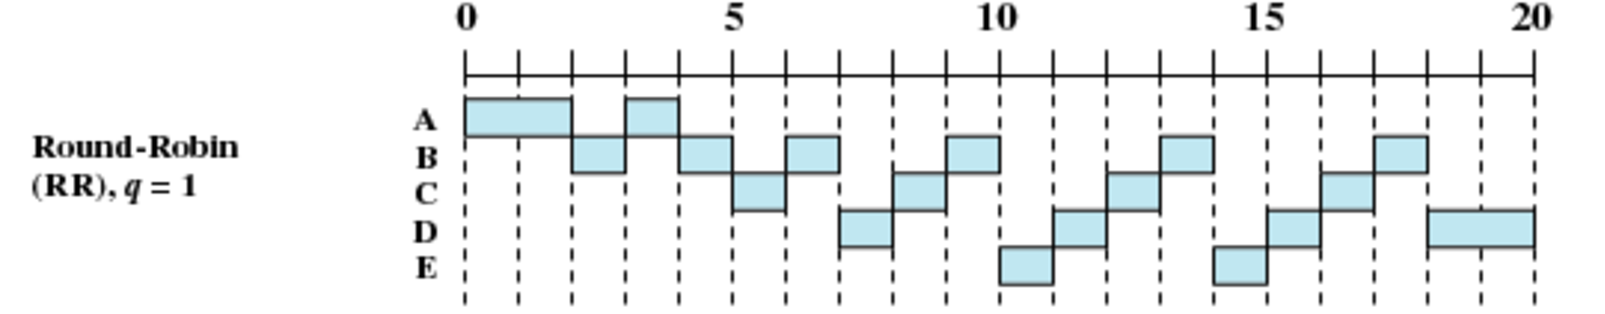
\includegraphics[width=\textwidth]{rr.pdf}
\end{minipage}
\newline

\begin{minipage}{0.8 \textwidth}
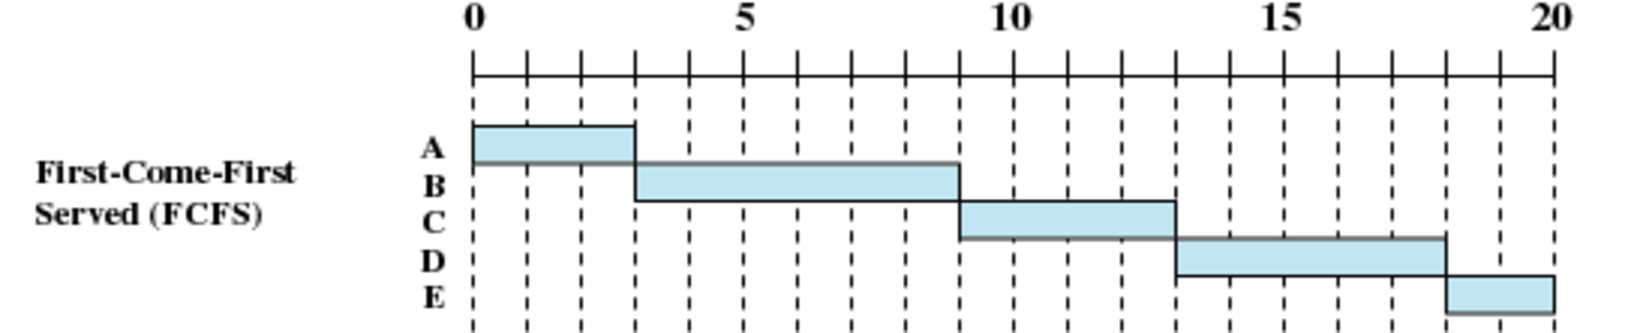
\includegraphics[width=\textwidth]{fcfs.pdf}
\end{minipage}
\newline

\begin{minipage}{0.8 \textwidth}
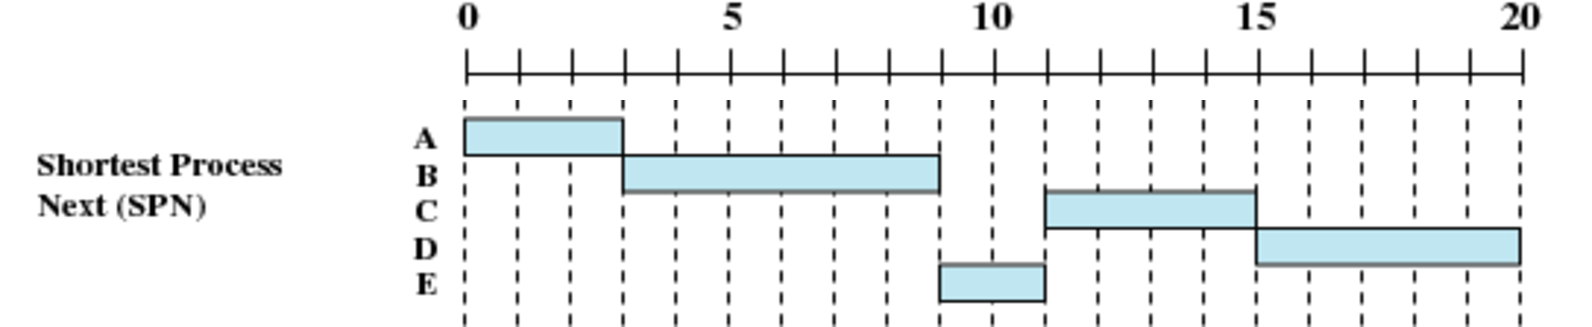
\includegraphics[width=\textwidth]{spn.pdf}
\end{minipage}
\newline

\begin{minipage}{0.8 \textwidth}
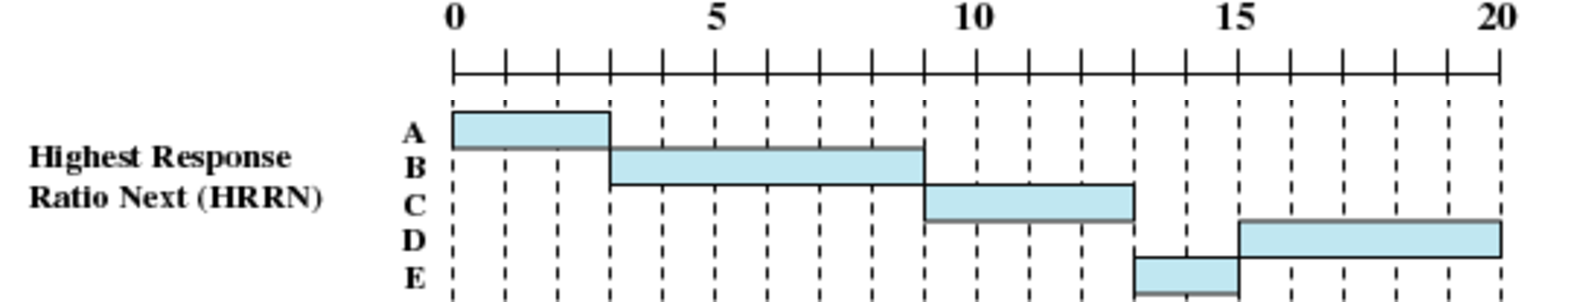
\includegraphics[width=\textwidth]{hrrn.pdf}
\end{minipage}
\newline

Bei unserem 3. Test kommen alle Prozesse (theoretisch) zur gleichen Zeit in die Queue und haben auch die gleichen voraussichtlichen Ausführungzeiten. Bei Round-Robin ergibt sich die übliche geschachtelte Ausführung, während sich für die nicht-präventiven Scheduling-Algorithmen wieder die drei gleichen Ausführungsreihenfolgen ergeben und zwar derart, dass die Prozesse in ihrere Reihenfolge in der Prozessliste abgearbeitet werden. Für FCFS ist das klar, denn FCFS wählt einfach den ersten Prozess aus der Prozessliste, der noch zu absolvierenden Zyklen hat. Für SPN und HRRN ebenso, denn die Scores zur Auswahl der Prozesse sind bei allen Prozessen der Liste gleich, die Prozessliste wird von vorne nach hinten iteriert und sofern kein Prozess mit noch auszuführenden Zyklen gefunden wird, der einen niedrigeren, bzw. höheren Score erzielt, wird der aktuell zur Ausführung ausgewählte Prozess beibehalten. Das führt aber gerade zur FCFS-Ausführungreihenfolge.


\end{document}
